%%% spell check: 
%%%% handouts:  pdfjam --landscape --nup '2x2' ecology1.pdf


%%% PRIOR TO CLASS: have all participants download the class data into
%%% a working directory on their computer; make sure all computers
%%% have a current version of R

%\documentclass[handout]{beamer}
\documentclass[10pt]{beamer}
\usepackage{parskip}
\usepackage{fancyvrb}
\usepackage{graphicx}
\setlength{\parskip}{1.75ex}

\mode<presentation>
{\usetheme{Singapore}
\setbeamercovered{transparent}}

\title{R Minicourse Workshop\\White River Case Study}

\author{\small Presented to the\\
        Washington State Deptment of Ecology\\
       September 2--3, 2014}

\date{\scriptsize Dr.~Robin Matthews, Institute for Watershed Studies\\
   Dr. Geoffrey Matthews, Computer Science Department\\
   Western Washington University}


\setbeamertemplate{blocks}[rounded][shadow=true]
\setbeamertemplate{footline}{\hspace*{5ex}Part 1 - Sept.~2, 2014 
   \hfill Page \insertframenumber \hspace{0.1ex} of
   \inserttotalframenumber \hspace*{5ex}
   \vspace*{2ex}}

\newcommand{\red}{\color{red}}
\newcommand{\blue}{\color{blue}}
\newcommand{\iwsframe}[2]{
\begin{frame}[fragile]
\frametitle{#1}
\framesubtitle{#2}
}

\begin{document}

\newcommand{\be}{\begin{enumerate}}
\newcommand{\ee}{\end{enumerate}}
\newcommand{\bi}{\begin{itemize}}
\newcommand{\ei}{\end{itemize}}
\newcommand{\bd}{\begin{description}}
\newcommand{\ed}{\end{description}}


\begin{frame}
\titlepage
\end{frame}

\iwsframe{White River Case Study}{Preliminaries}
\bi
\item The R scripts for this lecture are called {\tt \blue whiteriver01.r}
  and {\tt \blue whiteriver02.r}.
\item The first script does one reach, distance, and parameter,
  interactively.
\item  The second
  does all combinations of reach, distance, and several
  parameters and saves the results into files. {\tt \blue
    whiterivertext.txt} and {\tt \blue whiteriverplot.pdf}
\item Greg Pelletier provided a spreadsheet
{\blue  \verb|Q2KW_White_River_observed_and_predicted_data.xlsx|}
\item I saved the two pages of the spreadsheet into two  csv files:
\bi
\item{\blue \verb|Q2KW_White_River_observed_data.csv|}
\item{\blue \verb|Q2KW_White_River_predicted_data.csv|}
\ei
\ei

\end{frame}


\iwsframe{White River Case Study}{Loading the Data} 
\VerbatimInput[fontsize=\scriptsize,firstline=12,lastline=26,formatcom=\red]{whiteriver01.r}

\end{frame}


\iwsframe{White River Case Study}{Large size of the dataset makes it hard to view interactively.}

\begin{Verbatim}[fontsize=\scriptsize,commandchars=\\\{\}]
\red dim(observed)
\blue [1] 47265    54
\red dim(predicted)
\blue [1] 48450    79
\red names(observed)
\blue [1] "Reach.number" 
\blue [2] "Distance..Km."                     
\blue [3] "Date.time"
\blue [4] "Temperature..degC."                
\blue [5] "Conductivity..uS.cm.25C." ...
\red names(predicted)
\blue [1] "Reach"
\blue [2] "Distance..Km." 
\blue [3] "Date.time"     
\blue [4] "Temperature..degC."  
\blue [5] "Conductivity..uS.cm.25C." ...
\end{Verbatim}
\end{frame}


\iwsframe{White River Case Study}{Observed {\em vs.} predicted reaches}
\bi
\item We want to use reach and distance as a site.
\item Examining reaches in both observed and predicted shows
that the observed reaches are a subset of the predicted reaches.
\item So we can use the same reach, {\em e.g.} 23, for both files.
\ei
\begin{Verbatim}[fontsize=\scriptsize,commandchars=\\\{\}]
\red observed.reaches <- unique(sort(observed\$Reach.number))
\red observed.reaches
\blue [1]  3  8 13 20 21 22 23 25 27 28 31 33
\red predicted.reaches <- unique(sort(predicted\$Reach))
\red predicted.reaches
\blue [1]  0  1  2  3  4  5  6  7  8  9 10 11 12 13 14 15 16 17 18 19 20 21 22 23 24 25 26 27 28 29 30 31 32 33
\red my.reach <- 23
\end{Verbatim}
\end{frame}


\iwsframe{White River Case Study}{Observed {\em vs.} predicted
  distances}
\bi
\item Distances are not the same in the two files.
\item We will have to find a closest distance in the predicted file to
  match any distance in the observed file.
\ei
\begin{Verbatim}[fontsize=\scriptsize,commandchars=\\\{\}]
\red observed.distances
\blue [1]  0.03574664  2.15476664  5.81305664  7.90000000  9.37570664 12.01200000 13.31981664 16.00000000
\blue [9] 24.72141000 31.85200000 39.69900000
\red predicted.distances
\blue [1]  0.04  1.12  2.15  3.35  4.51  5.81  7.09  8.28  9.38 10.72 11.83 13.32 15.25 16.20 17.05 18.62 19.69
\blue [18] 20.75 22.08 23.44 24.72 26.12 27.46 28.73 30.23 31.85 33.58 34.85 36.57 38.21 39.70 41.00 42.56 44.14
\red my.observed.distance <- observed.distances[6]
\red min.difference.index <- which.min(abs(predicted.distances - my.observed.distance))
\red my.predicted.distance <- predicted.distances[min.difference.index]
\end{Verbatim}
\end{frame}


\iwsframe{White River Case Study}{Parameter names and columns}

\begin{Verbatim}[fontsize=\scriptsize,commandchars=\\\{\}]
\red observed.parameter.name <- "pH"
\red observed.parameter.column <- which(names(observed) == observed.parameter.name)
\red predicted.parameter.name <- "pH"
\red predicted.parameter.column <- which(names(predicted) == predicted.parameter.name)
\end{Verbatim}

\bi
\item
Now we can use any of the following:
\bi
\item\red \verb|observed[[observed.parameter.column]]|
\item \verb|observed[,observed.parameter.column]|
\item \verb|observed$pH|
\item \verb|observed[[observed.parameter.name]]|
\ei
\item
And similarly for \red\verb|predicted|
\ei
\end{frame}
\iwsframe{White River Case Study}{Creating an ID for selected parameter, reach, distance}
\bi
\item We have now selected a parameter, a reach, and a distance.
\item It will be helpful to print these out here and there, so we make
a string with all this information in it.
\ei
\VerbatimInput[fontsize=\scriptsize,firstline=75,lastline=78,formatcom=\red]{whiteriver01.r}
\end{frame}
\iwsframe{White River Case Study}{Selecting the rows}
\bi
\item We want only the data from the selected reach and distance,
  which also has a valid date and a valid datum.
\item So we select just those rows.
\item If the number of rows is too small, we can try a different
reach and distance.
\item Note that reach has different names in the two datasets.
\ei
\begin{Verbatim}[fontsize=\scriptsize,commandchars=\\\{\}]
\red observed.rows <- (observed\$Reach.number == my.reach) & 
\red   (observed\$Distance == my.observed.distance) &
\red   (!is.na(observed\$Date.time)) &
\red   (!is.na(observed[,observed.parameter.column]))

\red predicted.rows <- (predicted\$Reach == my.reach) & 
\red   (predicted\$Distance == my.predicted.distance) &
\red   (!is.na(predicted\$Date.time))&
\red   (!is.na(predicted[,predicted.parameter.column]))
\end{Verbatim}
\end{frame}

\iwsframe{White River Case Study}{Subsetting the rows and columns of the data}
\bi
\item We can now select just the rows and columns we want.
\item This will be the data we analyze, it has been ``cleaned'' so
  that we don't have to worry about missing numbers, {\em etc.}
\ei
\begin{Verbatim}[fontsize=\scriptsize,commandchars=\\\{\}]
\red date.name <- "Date.time"
\red observed.date.column <- which(names(observed) == date.name)
\red predicted.date.column <- which(names(predicted) == date.name)
\red 
\red observed.columns <- c(observed.date.column, observed.parameter.column)
\red predicted.columns <- c(predicted.date.column, predicted.parameter.column)
\red 
\red observed.subset <- observed[observed.rows, observed.columns]
\red predicted.subset <- predicted[predicted.rows, predicted.columns]
\end{Verbatim}
\end{frame}

\iwsframe{White River Case Study}{Plotting observed and predicted data}
\bi
\item We want plots of observed and predicted to have the same $x$ and
  $y$ range, so we find the biggest range needed for each.
\ei
\begin{Verbatim}[fontsize=\scriptsize,commandchars=\\\{\}]
\red x.range <- as.numeric(range(c(observed.subset$Date.time,
\red                              predicted.subset$Date.time)))
\red y.range <- range(c(observed.subset[[observed.parameter.name]],
\red                   predicted.subset[[predicted.parameter.name]]))
\end{Verbatim}
\bi
\item Now we can plot the data.
\ei
\VerbatimInput[fontsize=\scriptsize,firstline=113,lastline=118,formatcom=\red]{whiteriver01.r}
\end{frame}

\iwsframe{White River Case Study}{Observed plot}
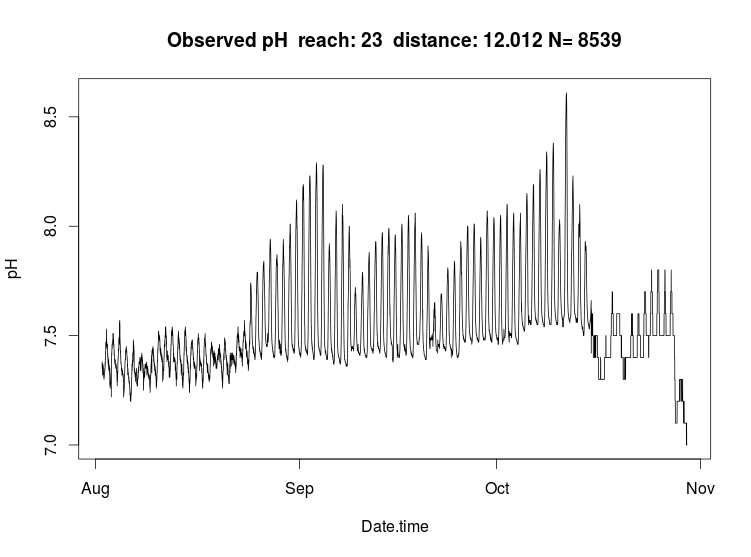
\includegraphics[width=\textwidth]{whiteriverplot01.png}
\end{frame}

\iwsframe{White River Case Study}{Predicted plot}
\VerbatimInput[fontsize=\scriptsize,firstline=119,lastline=124,formatcom=\red]{whiteriver01.r}
\end{frame}

\iwsframe{White River Case Study}{Predicted plot}
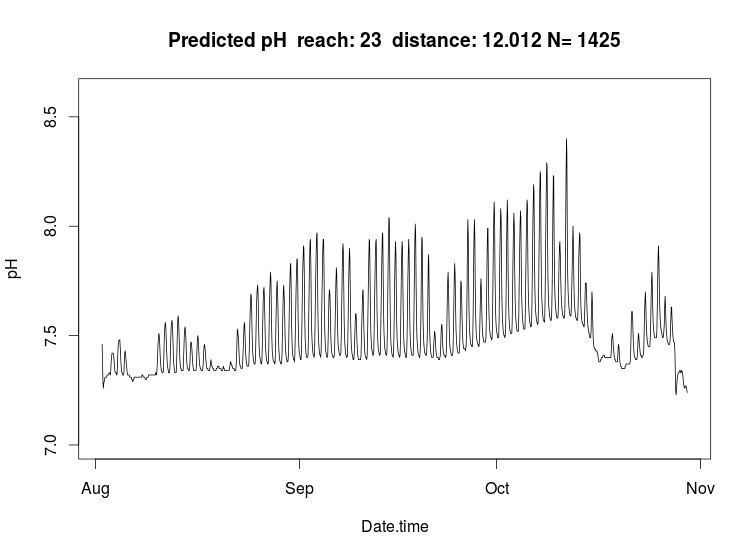
\includegraphics[width=\textwidth]{whiteriverplot02.png}
\end{frame}

\iwsframe{White River Case Study}{Predicted and observed plot}
\VerbatimInput[formatcom=\red,fontsize=\scriptsize,firstline=136,lastline=148]{whiteriver01.r}
\end{frame}


\iwsframe{White River Case Study}{Predicted and observed plot}
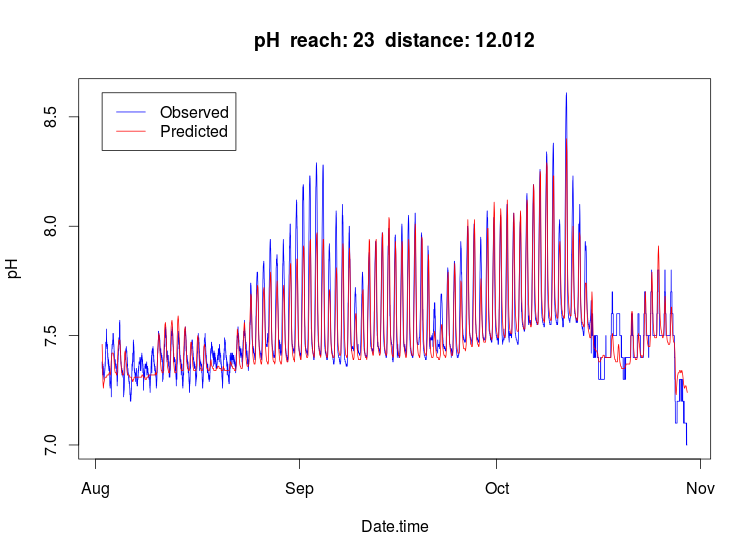
\includegraphics[width=\textwidth]{whiteriverplot03.png}
\end{frame}

\iwsframe{White River Case Study}{Subsample the data}
\bi
\item There are tens of thousands of rows for some of these plots.
\item We make analysis more tractable by subsampling.
\ei
\VerbatimInput[formatcom=\red,fontsize=\scriptsize,firstline=158,lastline=166]{whiteriver01.r}
\end{frame}


\iwsframe{White River Case Study}{Plot the observed and predicted subsample}
\VerbatimInput[formatcom=\red,fontsize=\scriptsize,firstline=184,lastline=197]{whiteriver01.r}
\end{frame}


\iwsframe{White River Case Study}{Plot the observed and predicted subsample}
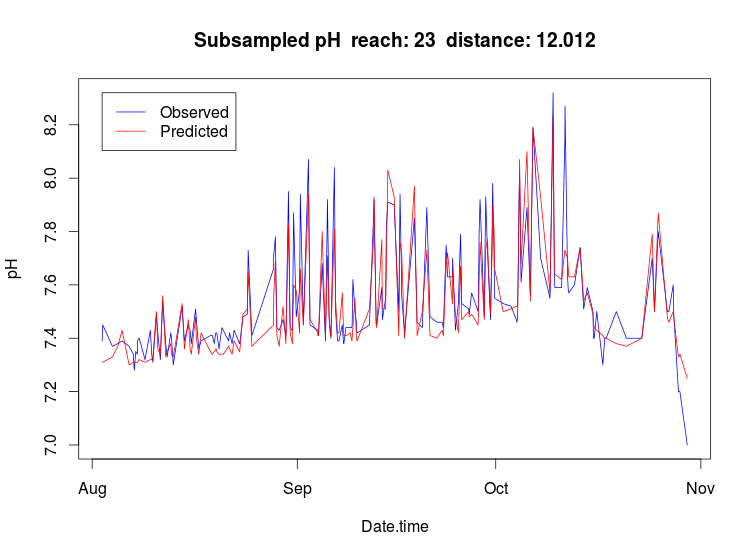
\includegraphics[width=\textwidth]{whiteriverplot04.png}
\end{frame}

\iwsframe{White River Case Study}{Fit a linear model}
\begin{Verbatim}[fontsize=\scriptsize,commandchars=\\\{\}]
\red my.model <- lm(predictions ~ observed.sample[[observed.parameter.name]])
\red summary(my.model)
\blue Call:
\blue lm(formula = predictions ~ observed.sample[[observed.parameter.name]])
\blue 
\blue Residuals:
\blue      Min       1Q   Median       3Q      Max 
\blue -0.25823 -0.03804 -0.00541  0.04324  0.24426 
\blue 
\blue Coefficients:
\blue                                            Estimate Std. Error t value Pr(>|t|)    
\blue (Intercept)                                 1.26902    0.19073   6.653 2.74e-10 ***
\blue observed.sample[[observed.parameter.name]]  0.82893    0.02526  32.815  < 2e-16 ***
\blue ---
\blue Signif. codes:  0 ‘***’ 0.001 ‘**’ 0.01 ‘*’ 0.05 ‘.’ 0.1 ‘ ’ 1
\blue 
\blue Residual standard error: 0.07581 on 198 degrees of freedom
\blue Multiple R-squared:  0.8447,	Adjusted R-squared:  0.8439 
\blue F-statistic:  1077 on 1 and 198 DF,  p-value: < 2.2e-16
\end{Verbatim}
\end{frame}


\iwsframe{White River Case Study}{Plot the observed {\em vs.}
  predicted and the linear fit}
\VerbatimInput[formatcom=\red,fontsize=\scriptsize,firstline=205,lastline=214]{whiteriver01.r}
\end{frame}

\iwsframe{White River Case Study}{Plot the observed {\em vs.}
  predicted and the linear fit}
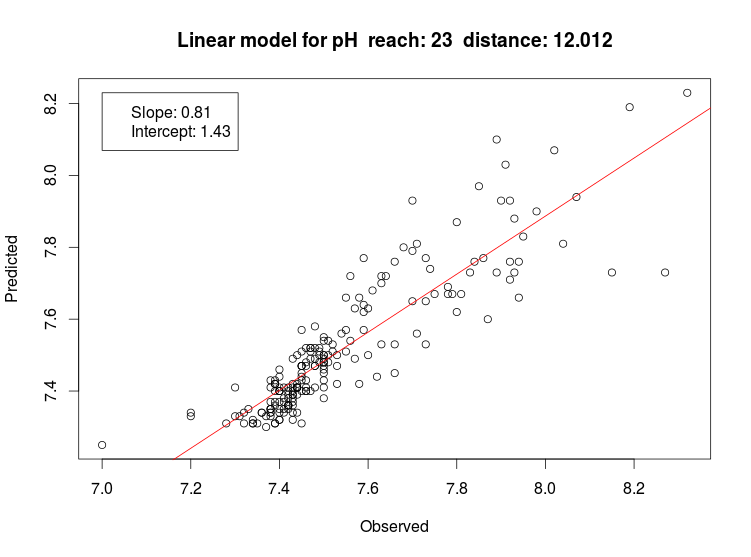
\includegraphics[width=\textwidth]{whiteriverplot05.png}
\end{frame}


\iwsframe{White River Case Study}{ANOVA on the model}
\begin{Verbatim}[fontsize=\scriptsize,commandchars=\\\{\}]
\red anova(my.model)
\blue Analysis of Variance Table
\blue 
\blue Response: predictions
\blue                                             Df Sum Sq Mean Sq F value    Pr(>F)    
\blue observed.sample[[observed.parameter.name]]   1 6.1881  6.1881  1076.8 < 2.2e-16 ***
\blue Residuals                                  198 1.1378  0.0057                      
\blue ---
\blue Signif. codes:  0 ‘***’ 0.001 ‘**’ 0.01 ‘*’ 0.05 ‘.’ 0.1 ‘ ’ 1
\end{Verbatim}
\end{frame}

\iwsframe{White River Case Study}{Plot the residuals for the linear model}
\begin{Verbatim}[fontsize=\scriptsize,commandchars=\\\{\}]
\red par(mfrow=c(2,2))
\red plot(my.model, main=my.id)
\red par(mfrow=c(1,1))
\end{Verbatim}
\end{frame}

\iwsframe{White River Case Study}{Plot the residuals for the linear model}
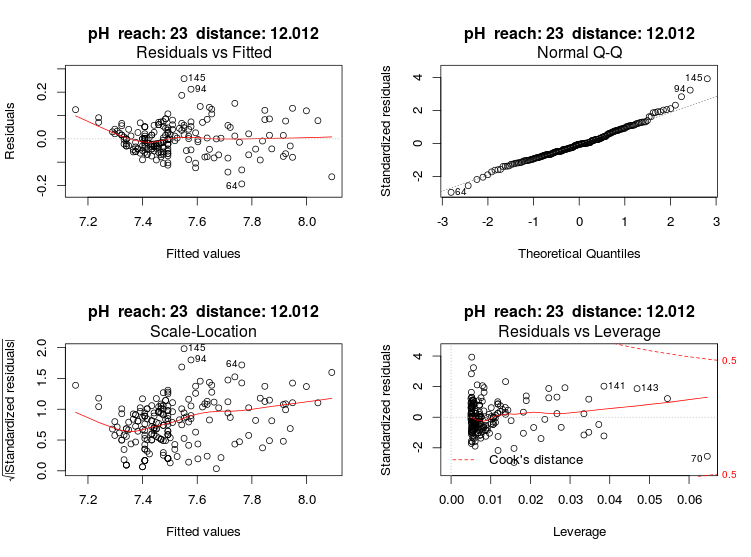
\includegraphics[width=\textwidth]{whiteriverplot06.png}
\end{frame}


\end{document}
\end
